\documentclass[11pt]{article}
\usepackage[a4paper,margin=2.5cm]{geometry}
\usepackage[T1]{fontenc}
\usepackage{booktabs}
\usepackage{graphicx}
\usepackage{hyperref}
\usepackage{natbib}

\title{Saal Baad, Mila Kar: Small Local ReAct Agents Lose Up to a Third of Their Accuracy on Roman Urdu Clinic Questions}
\author{Muzammal Hussain\\Masmatix Innovations, Glasgow, United Kingdom\\\texttt{muzammal@masmatixinnovations.co.uk}}
\date{Draft, November 2026}

\begin{document}
\maketitle

\begin{abstract}
Tool-using agents built on small language models can run on a clinic's own computer, but their users in Pakistan and in Pakistani communities in the UK often type in Roman Urdu: Urdu written in Latin script, without a fixed spelling. We ask how much accuracy a ReAct agent loses on Roman Urdu, which words cause the loss, and whether two cheap fixes help. We built 96 questions over a fictional physiotherapy clinic from 12 templates, each in English, common Roman Urdu spelling and chat spelling, with gold answers computed from the records, and ran four local models (Qwen2.5 3B and 7B, Llama 3.2 3B, Llama 3.1 8B) at temperature 0, for 3,838 scored calls. With an English worked example, ReAct accuracy fell from English to Roman Urdu by 34.7 points for Qwen2.5 3B, 31.2 for Llama 3.2 3B and 21.9 for Llama 3.1 8B (95\% bootstrap intervals all below zero), while Qwen2.5 7B showed no loss (+1.0). Chat spelling cost Qwen2.5 3B a further 22.1 points. The largest losses were on time words (\emph{saal baad}, \emph{saal pehle}), \emph{mila kar} (combined) and clinic days. For the two Llama models, answering with the whole database in the prompt showed no Roman Urdu gap, so the loss appeared inside the agent loop. A Roman Urdu worked example and translating the question first helped Llama 3.2 3B (+16.7 and +20.8 points) but not Qwen2.5 3B. A pilot also showed that sending the ReAct transcript as one user message, instead of separate chat turns, dropped Llama 3.2 3B to 7\% in English. Code, items and every call with its transcript are public.
\end{abstract}

\section{Introduction}
ReAct \citep{yao2023react} lets a language model alternate between a thought, a tool call and the tool's observation until it can answer. The pattern is simple enough to run with small open models on a laptop, which matters for clinics that cannot send patient questions to a hosted service. Most agent evaluations, however, are in English, and multilingual reasoning results such as MGSM \citep{shi2023mgsm} use native scripts rather than the romanised, code-mixed text that many South Asian users actually type.

Roman Urdu is a hard case for a small model. The same word is spelled several ways (\emph{zyada}, \emph{ziada}; \emph{baqi}, \emph{baki}), and short phrases decide the arithmetic: \emph{5 saal baad} means add five years, \emph{5 saal pehle} means subtract them. An agent that misreads one of them can still call the right tools and return a confident, wrong number. In an earlier 12-question pilot by the author, changing only the patient names moved one model's Roman Urdu ReAct accuracy from 83\% to 58\%, with errors on exactly these phrases.\footnote{\url{https://github.com/MHKhan50/agentic-ai-research-log/tree/main/react-roman-urdu}} This paper repeats the question at a size that supports confidence intervals.

We ask four questions. (1) Do small local agents answer clinic questions less accurately in Roman Urdu than in English? (2) Which question types cause the gap? (3) How much do surface changes move accuracy: other names with identical numbers, and chat spelling? (4) Do two cheap fixes help: a Roman Urdu worked example, or translating the question into English first? Our contributions are a public, templated benchmark with paired English and Roman Urdu forms and computed gold answers; a paired comparison across four local models and four methods; an error analysis by question type and by step type; and a protocol finding about how the agent loop is presented to a chat model.

\section{Related work}
\paragraph{Tool-using agents.} ReAct \citep{yao2023react} interleaves reasoning traces with actions and observations and is the basis of many agent frameworks. We use its loop unchanged, with three tools, and vary only the input language, the worked example and the model.

\paragraph{Multilingual and code-switched reasoning.} \citet{shi2023mgsm} translated grade-school maths problems into ten languages and found that chain-of-thought reasoning works across languages for large models, with lower accuracy in less represented languages. Code-switched benchmarks such as GLUECoS \citep{khanuja2020gluecos} show accuracy losses on text that mixes two languages. Roman Urdu combines both difficulties: it mixes Urdu and English and has no standard spelling.

\paragraph{Translating first.} Translate-test, translating the input into English and running an English system, can be strong when translation is good \citep{artetxe2023revisiting}. We test the cheap version available on a laptop: the same small model translates the question before running the English agent.

\section{Benchmark and method}
\paragraph{Clinic and items.} A fictional physiotherapy clinic has six patients and three therapists. Twelve templates cover the operator words that caused errors in the pilot (Table~\ref{tab:templates}): sessions remaining (\emph{baqi}), pain drop (\emph{kam hua}), age after and before $N$ years (\emph{saal baad}, \emph{saal pehle}), combined and difference in experience (\emph{mila kar}, \emph{zyada}), total sessions of a therapist's patients (two hops, \emph{kul}), a therapist's specialty and clinic days, percentage completed, sessions left after two more (\emph{agar \dots baqi}) and which of two patients did more sessions. Each template has four instances, and each instance exists with two name sets that share every number, giving 96 items. Gold answers are computed from the records in code. Each item has three forms: English, Roman Urdu with common spelling and Roman Urdu with chat spelling (for example \emph{kitnay}, \emph{sal}, \emph{pehlay}, \emph{ziada}, \emph{milakar}).

\paragraph{Methods.} \emph{Direct}: the whole database is in the system prompt and the model answers in one call. \emph{ReAct (English example)}: the model may call \texttt{lookup\_patient}, \texttt{lookup\_therapist} and \texttt{calculate} (arithmetic only), with one worked example in English; the code runs each tool and writes the real observation. On the Roman Urdu forms we add \emph{ReAct (Roman Urdu example)}, the same example written in Roman Urdu, and \emph{translate-then-ReAct}, where the model first translates the question into English and the English agent then runs; the translation is recorded. The agent has at most eight steps.

\paragraph{Models.} Qwen2.5 3B and 7B \citep{qwen2025qwen25} and Llama 3.2 3B and Llama 3.1 8B \citep{grattafiori2024llama3} ran through Ollama on a MacBook M4 with 16\,GB memory, with default quantisation, temperature 0 and seed 42. Each model answered 960 calls (96 items; two methods on English and four on each Roman Urdu form). Two of the 3,840 calls timed out twice after five minutes and are excluded (Qwen2.5 3B, one Roman Urdu ReAct call; Llama 3.1 8B, one Roman Urdu-example call).

\paragraph{Scoring and diagnostics.} An answer is correct (lenient) if any number in it matches the gold value (tolerance 0.01, one point for percentages); the strict score requires the last number to match. Number words up to twenty are read in English and Urdu, and text answers use keyword groups (therapist names, specialties, English and Urdu day names); for ``who did more'' the right name must come first. For ReAct runs we also record a wrong arithmetic operator (for example a minus for \emph{saal baad}), fewer lookups than the question needs, format errors, step-limit hits and latency.

\paragraph{Statistics.} Accuracies have Wilson 95\% intervals \citep{wilson1927}. Differences between forms or methods are paired on the same items, with a 95\% interval from 2,000 bootstrap resamples of items \citep{efron1979bootstrap}.

\section{Results}
\begin{figure}[t]
\centering
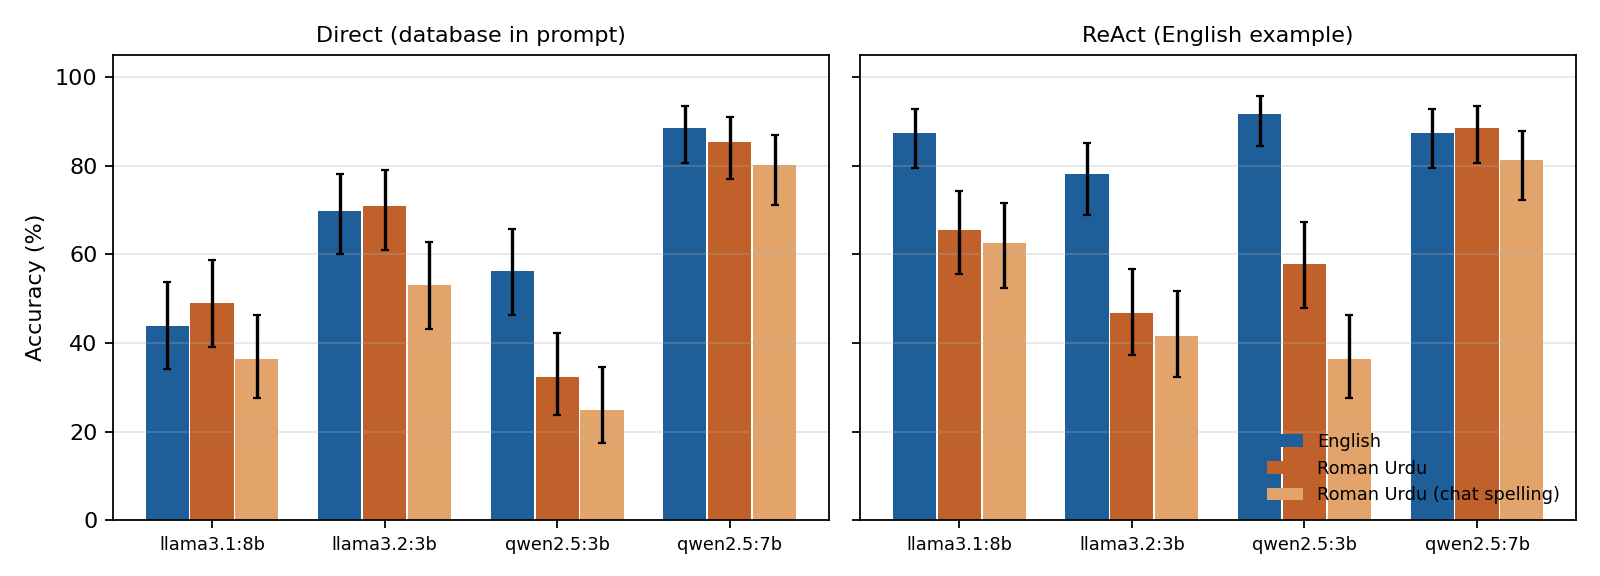
\includegraphics[width=\linewidth]{figures/fig_accuracy.png}
\caption{Accuracy (lenient) with Wilson 95\% intervals, 96 items per bar. Left: database in the prompt. Right: ReAct with an English worked example.}
\label{fig:acc}
\end{figure}

\begin{table}[t]
\centering
\small
\begin{tabular}{lrrrr}
\toprule
Model & English & Roman Urdu & Chat spelling & Roman Urdu $-$ English (95\% CI) \\
\midrule
Qwen2.5 3B & 91.7 & 57.9 & 36.5 & $-34.7$ [$-44.2$, $-25.3$] \\
Llama 3.2 3B & 78.1 & 46.9 & 41.7 & $-31.2$ [$-41.7$, $-19.8$] \\
Llama 3.1 8B & 87.5 & 65.6 & 62.5 & $-21.9$ [$-32.3$, $-11.5$] \\
Qwen2.5 7B & 87.5 & 88.5 & 81.2 & $+1.0$ [$-6.2$, $+7.3$] \\
\bottomrule
\end{tabular}
\caption{ReAct with an English worked example: accuracy (\%) by form, and the paired difference in percentage points.}
\label{tab:main}
\end{table}

\paragraph{The Roman Urdu gap.} With ReAct and an English example, three of the four models lost between 22 and 35 points on Roman Urdu, with intervals well below zero (Table~\ref{tab:main}, Figure~\ref{fig:acc}). Qwen2.5 7B lost nothing. Chat spelling added a further loss of 22.1 points [$-31.6$, $-13.7$] for Qwen2.5 3B, and smaller, non-significant losses for the others (3.1 to 7.3 points).

\paragraph{Direct answering.} With the whole database in the prompt, the two Llama models showed no Roman Urdu gap (Llama 3.1 8B $+5.2$ [$-7.3$, $+16.7$]; Llama 3.2 3B $+1.0$ [$-9.4$, $+11.5$]), but both lost clearly once they had to act as agents. For Llama 3.2 3B, ReAct was 24.0 points \emph{worse} than direct answering on Roman Urdu [$-37.5$, $-10.4$]. In English, ReAct helped Llama 3.1 8B (+43.8 points) and Qwen2.5 3B (+35.4), but not clearly Llama 3.2 3B (+8.3 [$-4.2$, $+21.9$]) or Qwen2.5 7B ($-1.0$), which was already at 88.5\% directly. Qwen2.5 3B lost accuracy on Roman Urdu with both methods (direct $-24.0$ [$-35.4$, $-13.5$]).

\begin{table}[t]
\centering
\small
\begin{tabular}{llrrr}
\toprule
Template & Key words & English & Roman Urdu & Chat spelling \\
\midrule
T01 sessions left & baqi & 88 & 81 & 84 \\
T02 pain drop & kam hua & 100 & 94 & 94 \\
T03 age in $N$ years & saal baad & 97 & 50 & 34 \\
T04 age $N$ years ago & saal pehle & 94 & 66 & 31 \\
T05 combined experience & mila kar & 100 & 56 & 47 \\
T06 experience difference & zyada & 100 & 100 & 78 \\
T07 two-hop total & kul & 94 & 75 & 66 \\
T08 therapist specialty & kaun, kya & 56 & 48 & 38 \\
T09 clinic days & kin dinon & 91 & 41 & 44 \\
T10 percent completed & kitna percent & 100 & 97 & 91 \\
T11 left after two more & agar \dots baqi & 56 & 34 & 28 \\
T12 who did more & kis ne zyada & 59 & 34 & 31 \\
\bottomrule
\end{tabular}
\caption{ReAct (English example) accuracy (\%) by question type, pooled over the four models (32 answers per cell).}
\label{tab:templates}
\end{table}

\paragraph{Which words.} Pooled over the four models (Table~\ref{tab:templates}), the largest drops were on the two time phrases (\emph{saal baad} 97\% to 50\%, \emph{saal pehle} 94\% to 66\%, and to 34\% and 31\% with chat spelling), on \emph{mila kar} (100\% to 56\%) and on clinic days (91\% to 41\%). \emph{Zyada} was read correctly in its common spelling (100\%) but less often as \emph{ziada} (78\%). Arithmetic-only questions such as percentage completed barely changed. The step diagnostics agree: in Roman Urdu, wrong operators rose from 0\% to 12.5\% for Llama 3.2 3B and to 8.4\% for Qwen2.5 3B, and Qwen2.5 3B skipped a required lookup in 8.4\% of Roman Urdu runs against 4.2\% in English. Three types (T08, T11, T12) were below 60\% even in English, so their Roman Urdu figures say less about language.

\paragraph{Surface changes.} Swapping the name set while keeping every number moved English accuracy by at most 4.2 points for any model. On Roman Urdu the largest shift was $-18.8$ points for Llama 3.1 8B, with an interval that includes zero [$-37.5$, $+2.1$] on 48 items, so the pilot's large name effect was not confirmed at this size.

\paragraph{Two cheap fixes.} For Llama 3.2 3B, a Roman Urdu worked example raised Roman Urdu accuracy by 16.7 points [$+5.2$, $+29.2$] and translating first by 20.8 [$+9.4$, $+31.2$]. For Llama 3.1 8B the Roman Urdu example helped by 11.6 points [$0.0$, $+24.2$] and translation by 10.4 [$-2.1$, $+22.9$]. Neither fix helped Qwen2.5 3B ($-3.2$ and $-1.1$) or Qwen2.5 7B. No fix closed the gap for the weaker models.

\paragraph{Protocol pilot.} Our first run sent the system prompt and the whole ReAct transcript as a single user message at every step. Qwen2.5 3B handled this (89.6\% in English, 96 items), but Llama 3.2 3B repeated its first step until the step limit in 93\% of English runs and scored 7.1\% (56 items before we stopped the run). With the same prompts, tools and grading, sending each model step as an assistant turn and each observation as a user turn raised Llama 3.2 3B to 78.1\%. All results above use the separate-turn format for every model; the pilot calls are kept in the repository.

\section{Discussion}
For three of four small local models, the same question in Roman Urdu cost a ReAct agent between a fifth and a third of its accuracy, and the losses were concentrated in short phrases that decide the arithmetic or the lookup. This matters for clinical tools because the failure mode is quiet: the agent still calls tools and returns a number. That the Llama models showed no gap when answering directly suggests that the multi-step loop, where a misread word can choose the wrong operator or skip a lookup, is where Roman Urdu does its damage; with four models we cannot say why Qwen2.5 3B was affected in both settings or why Qwen2.5 7B was not affected at all.

The protocol pilot is a warning for agent benchmarks in general: how the loop is presented to a chat model changed one model's English score from 7\% to 78\%, larger than any language effect we measured. Benchmarks should state this choice and, where possible, test both.

\section{Limitations}
The clinic is fictional and small, with 12 templates written by one person; real users spell Roman Urdu in more ways than our two forms. We tested four small open models with default quantisation, at temperature 0 with one sample per question. Lenient scoring can credit an answer that lists the right number among others; strict scores are within a few points except for Llama 3.2 3B's direct English answers (69.8\% lenient, 57.3\% strict). Three templates were hard even in English. The tools and system prompt were in English in every condition. Two calls were excluded after timeouts.

\section{Conclusion}
Small local ReAct agents that work well in English can lose up to a third of their accuracy on the same clinic questions in Roman Urdu, mostly on time and combination words, and chat spelling can make this worse. A larger model or, for some models, a Roman Urdu example or a translation step reduces the loss. Anyone deploying such agents for Roman Urdu users should test them in Roman Urdu, with the spellings their users type.

\section*{Data and code}
Items, code, tests, every call with its full transcript and the pilot run: \url{https://github.com/MHKhan50/agentic-ai-research-log/tree/main/roman-urdu-react-bench}.

\bibliographystyle{plainnat}
\bibliography{refs}
\end{document}
